\documentclass[11pt,a4paper]{article}
\usepackage[T1]{fontenc}
\usepackage[utf8]{inputenc}
\usepackage[margin=25mm]{geometry}
\usepackage{amsmath,amssymb,booktabs,array,graphicx}
\usepackage{xcolor}
\usepackage[colorlinks=true,linkcolor=blue,citecolor=blue,urlcolor=blue]{hyperref}
\usepackage{microtype}
\usepackage{caption}
\usepackage{pdflscape}
\captionsetup{font=small,labelfont=bf}
\setlength{\emergencystretch}{2em}
\newcommand{\tool}{Flash Silicon Analyzer}
\title{\textbf{Flash Silicon Analyzer:\\
An Inspectable Browser Tool for CMOS\\
Power, Performance, Area, Yield, and Cost Exploration}}
% Author name confirmed by the repository owner.
\author{Liang Dacheng}
\hypersetup{pdfauthor={Liang Dacheng},pdftitle={Flash Silicon Analyzer: An Inspectable Browser Tool for CMOS Power, Performance, Area, Yield, and Cost Exploration}}
\date{September 2026\\[3pt]\small Manuscript draft}
\begin{document}
\maketitle

\begin{abstract}
Early technology selection requires reasoning about logic density, memory
scaling, operating frequency, power, manufacturing yield, and cost together.
\tool{} implements this workflow as a self-contained HTML
application with an embedded process library and no external JavaScript
dependencies. Its 41 selectable entries cover six process families and combine
publicly motivated scaling factors with explicit estimation and roadmap
assumptions. The application separates logic, SRAM, and fixed area; evaluates
power at both source and estimated target frequencies; combines a
negative-binomial yield model with wafer, package/test, and amortized
non-recurring costs; and provides a deterministic rectangular-die wafer map,
including optional wafer-to-wafer stacking. We document the implemented
equations and reproduce experiments directly from the application's
JavaScript. For its default 400\,mm$^2$, 10\,W, 1\,GHz TSMC 12\,nm design,
the TSMC 6\,nm scenario produces 135.59\,mm$^2$, 6.178\,W at 1.20\,GHz,
79.03\% modeled yield, and \$36.07 per good die under the default cost
assumptions. Sensitivity experiments expose the effects of fixed area, SRAM,
wafer-cost basis, and stack yield. Arithmetic checks cover all 1,681
source--target combinations. These results establish reproducibility and
illustrate model behavior; they do not establish prediction accuracy against
measured silicon.
\end{abstract}

\section{Introduction}
Selecting a fabrication process changes more than transistor density. A
logic-dominated design can shrink substantially while its memory macros and
analog interfaces scale differently. A faster operating point can consume
more dynamic power than an equal-frequency comparison suggests. Higher wafer
cost and defect density can offset the benefit of a smaller die. A useful
early estimator must therefore expose the assumptions connecting power,
performance, area, and cost (PPAC), rather than reduce the decision to a
nominal node label.

This paper describes \tool{}, a browser application provided in the project
repository\footnote{\url{https://github.com/ldcyes/silicon_analysis}}.
The application accepts a reference design and a
source/target process pair, then displays estimated area, power, frequency,
yield, and cost. Its implementation is contained in one HTML file: the process
library, model functions, interface, and Canvas rendering are inspectable
together. A separate wafer-map view makes geometric edge losses and sampled
die failures visible.

Our contribution is a documented, reproducible integration of these
calculations. Specifically, we provide (i) a mathematical specification of
the implemented PPAC, yield, and cost paths; (ii) an architecture description
that distinguishes analytical estimates from the spatial wafer model; and
(iii) code-derived experiments and a source-provenance audit. The work does
not introduce a transistor model, a physical-design optimizer, or a new
statistical yield law. It does not report fabrication measurements, timing
signoff, predictive error against a held-out dataset, or performance
superiority over other tools.

\section{Background and relationship to prior work}
Stillmaker and Baas describe polynomial technology-scaling models derived from
HSpice simulations using PTM and ITRS inputs~\cite{stillmaker2017}.
Sarangi and Baas's DeepScaleTool fits published silicon data to estimate
area, delay, and energy scaling in the deep-submicron
regime~\cite{deepscale2021}. These works motivate source-to-target factor
ratios. \tool{} uses an explicit lookup table of normalized factors;
it does not reproduce their fitting procedures or inherit their reported
accuracy. In particular, this repository's 2\,nm-class and roadmap entries
extend beyond the process range studied by DeepScaleTool.

Negative-binomial defect models are part of a broader family of compound
statistical yield models. Bogdanov et al.\ discuss hierarchical fault
distributions across regions, wafers, and batches~\cite{yield2003}. The
present implementation uses a single negative-binomial survival expression
at each die location, with an optional radial adjustment. It does not model
the complete hierarchical distribution or generate spatially correlated
defect clusters.

Public foundry announcements provide some useful relative anchors. TSMC's
2019 N6 announcement states an 18\% logic-density improvement over
N7~\cite{tsmc2019}; the repository encodes this as $7.08/6.00=1.18$.
GlobalFoundries' 22FDX announcement describes FD-SOI and a 20\% smaller die
than 28\,nm~\cite{gf2015}; the corresponding density ratio in the library is
$1.25$, whose reciprocal is $0.8$. These examples check the interpretation of
two source statements. They do not validate every field in either record.

\section{Implementation and process-library provenance}
\label{sec:architecture}
Figure~\ref{fig:architecture} shows the evaluated application, identified by
the HTML SHA-256 recorded in Section~\ref{sec:experiments}. There is no
server-side model or persistent database. Input values are held in DOM
controls, while the process library and display state are JavaScript objects.
The page can be opened as a local file or served by any static HTTP server.
Clipboard access depends on browser permissions. Reloading the page restores
its defaults.

\begin{landscape}
\begin{figure}[p]
  \centering
  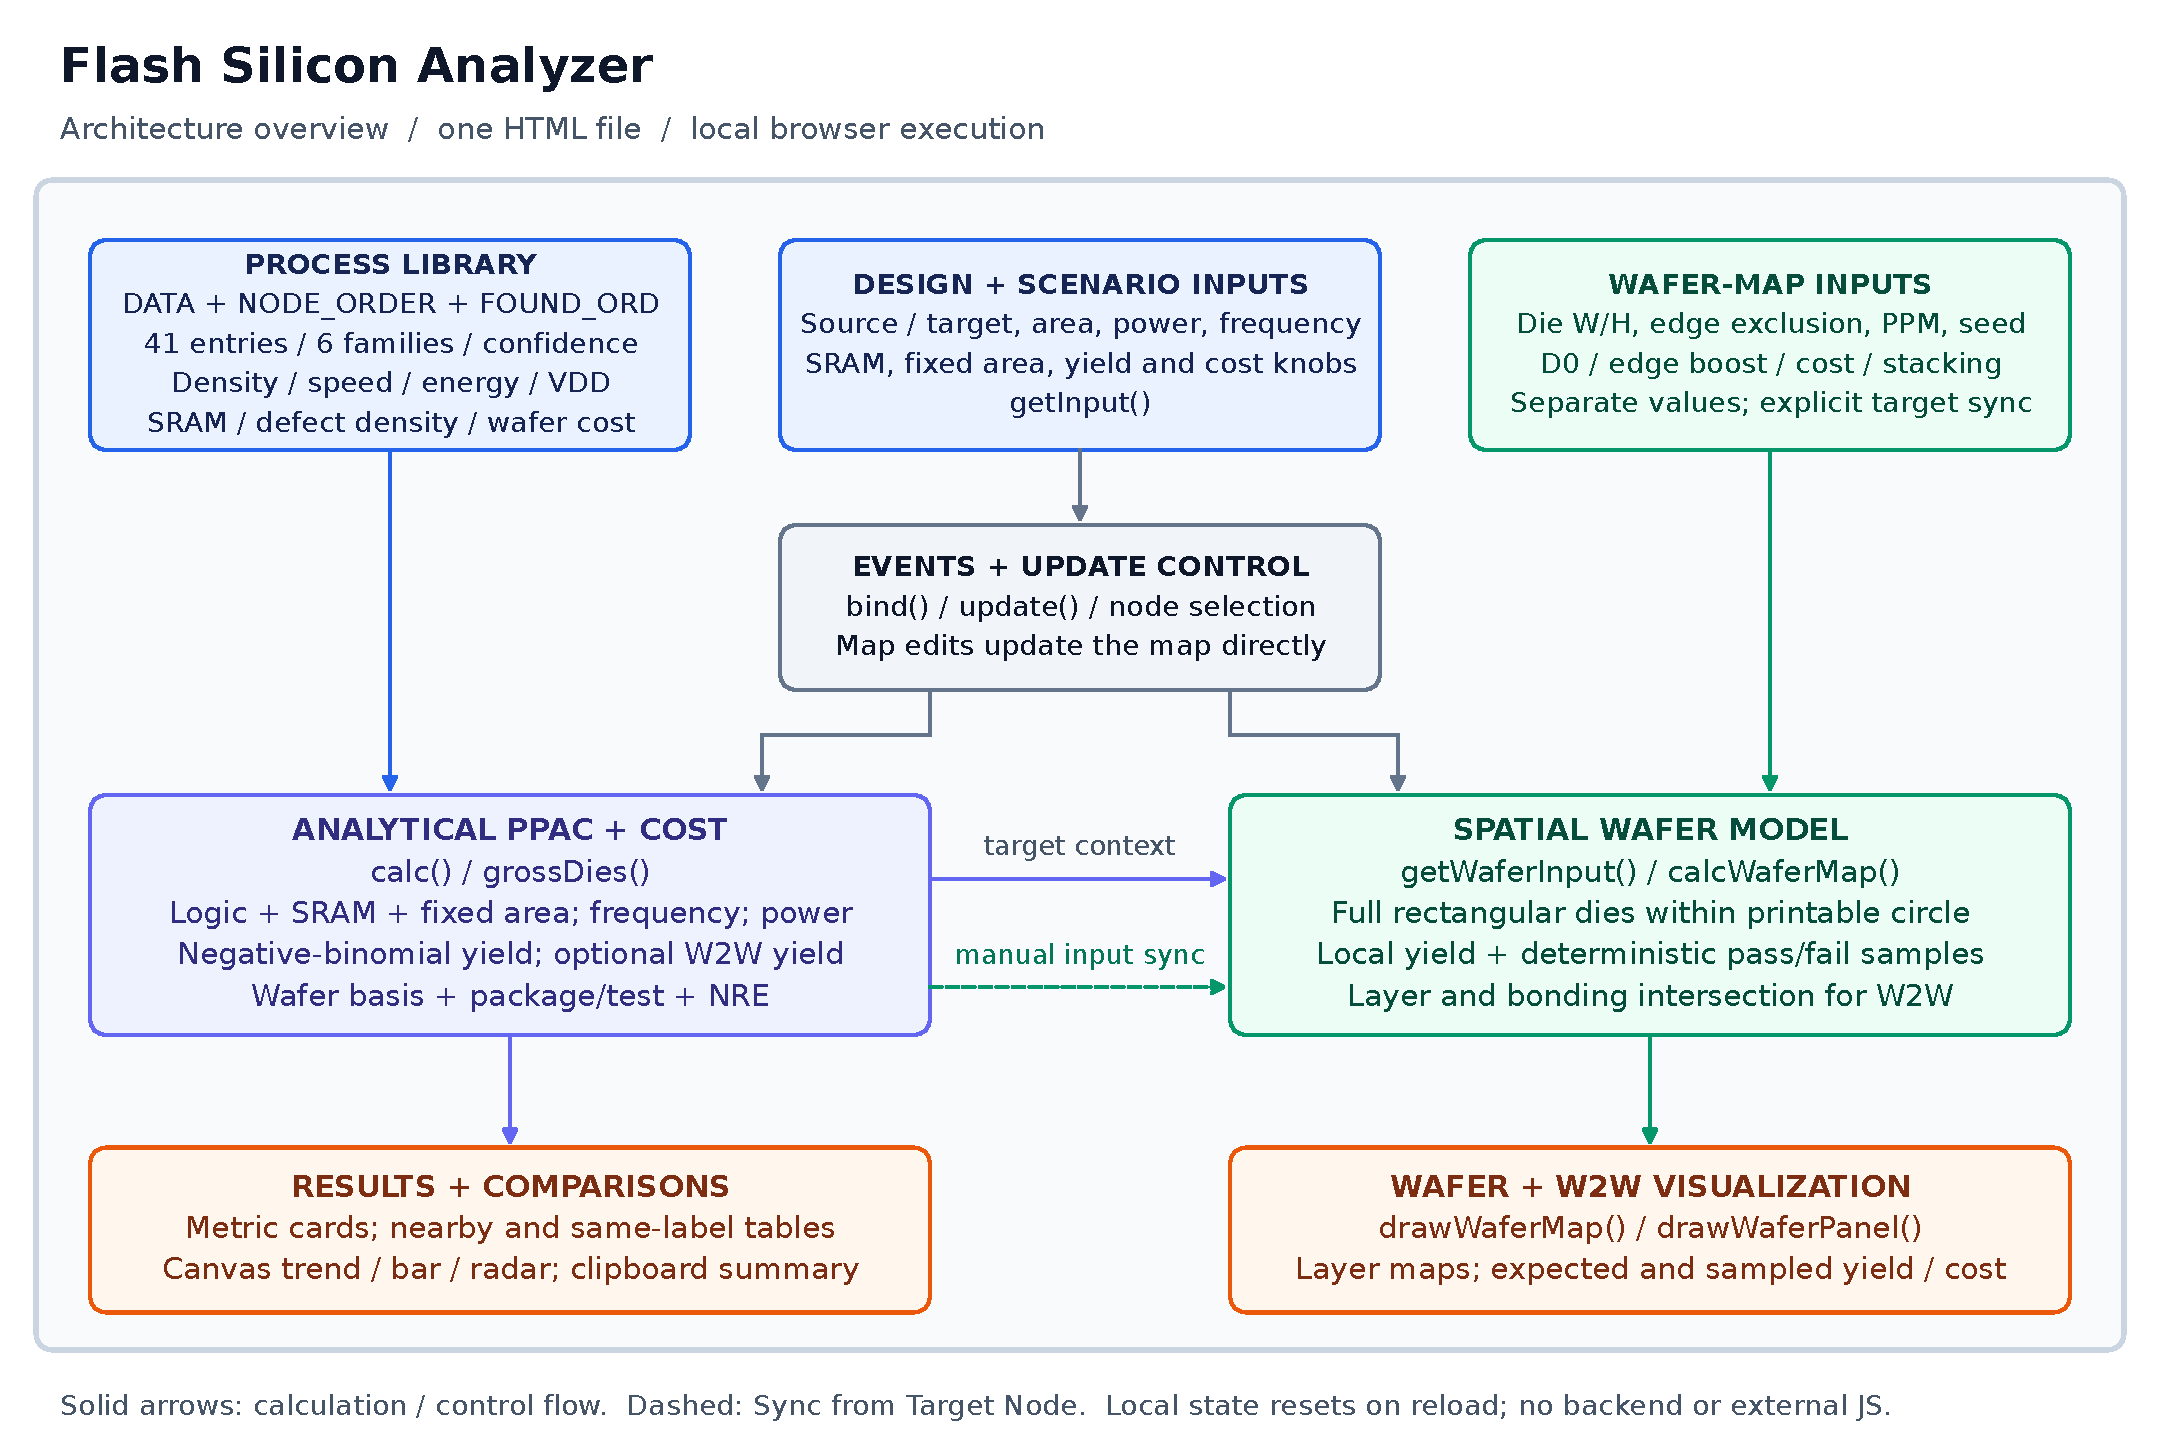
\includegraphics[width=\linewidth]{figures/architecture.pdf}
  \caption{Implemented browser architecture. Solid arrows show calculation or
  control flow. The dashed arrow denotes explicit copying of selected target
  values into the controls consumed by the wafer model. Map controls retain
  their own values between synchronizations. The editable source is
  \texttt{docs/architecture.drawio}.}
  \label{fig:architecture}
\end{figure}
\end{landscape}

\subsection{Model and presentation boundaries}
\texttt{getInput()} reads the main controls and \texttt{calc()} evaluates a
source--target pair. \texttt{update()} obtains the selected result and invokes
the metric-card, wafer-map, table, and chart updates. Trend charts repeat
\texttt{calc()} over the selected families and available nodes.
\texttt{nearbyNodes()} selects at most two neighboring entries on either side
in the foundry's supported-node sequence. Same-label comparisons include only
families containing that numeric label. The bar and radar plots normalize
values within the displayed comparison set; their scores are visual aids,
not absolute engineering objectives.

The map path uses \texttt{getWaferInput()} and \texttt{calcWaferMap()}.
Editing map controls recalculates that view directly. Main-input changes
refresh the map but do not automatically overwrite its width, height,
defect-density, or wafer-cost controls. The \emph{Sync from Target Node}
button copies selected values, including square-die dimensions derived from
target area. The dimensions are rounded to two decimals, $D_0$ to three,
and wafer cost to whole dollars. Edge exclusion, radial boost, extra failures
in parts per million (PPM), and random seed retain their current values.
Consequently, a refreshed map and the analytical cards need not describe
identical geometries or failure assumptions.

\subsection{Coverage and confidence labels}
Table~\ref{tab:coverage} reports the selectable library. The global order is
28, 22, 16, 14, 12, 10, 7, 6, 5, 4, 3, and 2. The keys are comparison labels,
not measured physical dimensions. Some records explicitly represent
interpolated classes or grouped process families, such as Intel
14++/12-class and 18A/20A-class. GlobalFoundries 22FDX remains a distinct
22\,nm FD-SOI record. Its missing advanced nodes are consistent with the
company's 2018 announcement placing its 7\,nm program on
hold~\cite{gf2018}; library coverage should not be interpreted as a current
foundry-service catalog.

\begin{table}[htbp]
\centering\small
\caption{Selectable process entries at the evaluated revision. H, M, and R
are the repository's High, Medium, and Roadmap labels.}
\label{tab:coverage}
\begin{tabular}{llrrrr}
\toprule
Family & Numeric labels & Count & H & M & R\\
\midrule
TSMC & 28,16,12,10,7,6,5,4,3,2 & 10 & 6 & 4 & 0\\
Samsung & 28,14,12,10,7,6,5,4,3 & 9 & 5 & 4 & 0\\
Intel & 14,12,10,7,4,3,2 & 7 & 5 & 2 & 0\\
SMIC & 28,14,7 & 3 & 1 & 2 & 0\\
GF & 28,22,14,12 & 4 & 3 & 1 & 0\\
Huawei $\tau$ & 14,10,7,6,5,4,3,2 & 8 & 0 & 1 & 7\\
\midrule
Total & & 41 & 20 & 14 & 7\\
\bottomrule
\end{tabular}
\end{table}

The availability predicate excludes records labeled \texttt{low} or
\texttt{alias}; it does not exclude every record whose descriptive text uses
mapping or interpolation. High and Medium are qualitative labels attached
to complete records, not field-level confidence intervals. A High record can
still include estimated power, defect-density, or cost parameters.

The HTML attributes wafer-cost baselines to previously uploaded IBS-style
tables and Huawei LogicFolding values to uploaded slides. Neither those
tables nor those slides are present in the evaluated repository. Their
titles, dates, and original contents therefore cannot be independently
checked from this artifact. We retain these numbers as repository assumptions
and do not cite a fabricated primary source for them. Similarly, the broad
TSMC, Samsung, Intel, and SMIC source descriptions in the interface are not
a field-by-field provenance record. The accompanying source ledger separates
verified contextual references from unsupported parameter provenance.

\section{Analytical model}
Unless specified otherwise, inputs are nonnegative physical quantities, with
strictly positive reference frequency, process factors, die area, and
clustering parameter. Numerical floors in the implementation prevent some
singular calculations; they do not replace complete input validation.

\subsection{Area and performance}
For process $p$, let $d_p$, $s_p$, and $e_p$ be normalized logic-density,
speed, and same-frequency dynamic-energy factors; let $m_p$ be SRAM density
in Mbit/mm$^2$ and $v_p$ the nominal supply voltage. Subscripts $s$ and $t$
refer to source and target processes. Given source logic area $A_{\ell,s}$,
SRAM capacity $M$, and fixed area $A_o$, the target estimate is
\begin{align}
A_{\ell,t} &= A_{\ell,s}\frac{d_s}{d_t}h_A, &
A_{m,t} &= \frac{M}{m_t}, \label{eq:area}\\
A_t &= \max(10^{-4},A_{\ell,t}+A_{m,t}+A_o),&
f_t &= f_s\frac{s_t}{s_s}h_f . \label{eq:freq}
\end{align}
SRAM area is zero when capacity is zero. $h_A$ is a logic-area overhead
factor and does not multiply SRAM or fixed area. $h_f$ is a user-selected
frequency-realization factor representing unmodeled implementation effects.
The term \emph{converged frequency} in the interface means this estimated
frequency; no timing-closure iteration is executed.

For most records the displayed standardized transistor density is
$15.3d_p$ MTr/mm$^2$, using a repository constant for the 28\,nm baseline.
Some Huawei records instead contain explicit standardized density, raw
density, and an effective density motivated by slide notes. Area uses
\texttt{density}, not the displayed standardized-density field. The
implemented $2/3$ conversion of Huawei raw MTR is a repository convention,
not a universal conversion between transistor-counting methods.

\subsection{Logic and SRAM power}
Let $P_{\ell,s}$ be the source logic-power input. Despite its \emph{active power}
label, the code assigns a fixed fraction $\lambda=0.08$ to leakage and the
remaining fraction to dynamic power. Define
\begin{align}
r_f &= f_t/f_s, &
r_e &= (e_t/e_s)h_P,\\
r_{\mathrm{leak}} &=
\max\left[0.08,
  \left(\frac{A_{\ell,t}}{A_{\ell,s}}\right)^{0.72}
  \left(\frac{v_t}{v_s}\right)^{1.2}\right], \label{eq:leak}\\
P_{\ell,\mathrm{same}} &=
(1-\lambda)P_{\ell,s}r_e+\lambda P_{\ell,s}r_{\mathrm{leak}},\\
P_{\ell,t} &=
(1-\lambda)P_{\ell,s}r_e r_f+\lambda P_{\ell,s}r_{\mathrm{leak}}.
\label{eq:power}
\end{align}
The implementation floors numerator and denominator logic areas at
$10^{-9}$ in Eq.~\ref{eq:leak}. The exponents, leakage fraction, and minimum
leakage scale are fixed heuristics; the repository contains no calibration
dataset for them. The power guardband $h_P$ acts on logic dynamic energy
only. It does not directly scale leakage or SRAM power.

When both $M>0$ and source SRAM dynamic power $P_{m,s}>0$, the SRAM contribution
is
\begin{equation}
P_{m,\mathrm{same}}=P_{m,s}\frac{m_s}{m_t}
\left(\frac{v_t}{v_s}\right)^2,\qquad
P_{m,t}=P_{m,\mathrm{same}}r_f .
\end{equation}
Otherwise it is zero. The displayed totals are
$P_{\mathrm{same}}=P_{\ell,\mathrm{same}}+P_{m,\mathrm{same}}$ and
$P_t=P_{\ell,t}+P_{m,t}$. Fixed-area blocks contribute no additional power.
The inverse-density SRAM power factor is an estimator heuristic, not a
macro-level energy model.

\subsection{Yield and cost}
For wafer diameter $D$ in mm, the analytical gross-die approximation is
\begin{equation}
G(A,D)=\max\left(0,\frac{\pi(D/2)^2}{A}
                   -\frac{\pi D}{\sqrt{2A}}\right). \label{eq:gross}
\end{equation}
The code returns zero when $A\leq0$. $G$ can be fractional, and the unrounded
value is used for cost. This approximation has no explicit die aspect ratio,
scribe street, reticle limit, or user-specified edge exclusion.

Let $A_c=A_t/100$ convert mm$^2$ to cm$^2$, $D_0$ be target defect density
in cm$^{-2}$ multiplied by a scenario factor $m_D$, and $\alpha>0$ be the
clustering parameter. With line/parametric yield $y_{\mathrm{line}}$,
\begin{equation}
Y_d=\left(1+\frac{D_0 A_c}{\alpha}\right)^{-\alpha},\qquad
q=Y_d y_{\mathrm{line}} . \label{eq:yield}
\end{equation}
For a conventional record, final yield is $q$. For a stack-enabled Huawei
record with $L\in\{2,3\}$ layers and bonding yield $b$ per interface,
\begin{equation}
Y_L=q^L b^{L-1}. \label{eq:stack}
\end{equation}
This assumes identical layer footprints and yields and independent layer
and bonding failures. It does not include known-good-die selection or repair.
Changing the layer selector changes yield and wafer multiplicity; it does
not independently improve the record's area, frequency, or power factors.

Let $W$ be the selected per-wafer baseline, $m_C$ a wafer-cost multiplier,
$P_{\mathrm{pkg}}$ package/test cost per good die, $N_{\mathrm{NRE}}$
non-recurring engineering expense, and $V$ production volume. Then
\begin{equation}
C_{\mathrm{Si}}=\frac{L W m_C}{G(A_t,D)Y_L},\qquad
C_{\mathrm{good}}=C_{\mathrm{Si}}+P_{\mathrm{pkg}}
                       +\frac{N_{\mathrm{NRE}}}{\max(1,V)}. \label{eq:cost}
\end{equation}
For conventional records set $L=1$. Zero gross dies or zero final yield
produce infinite silicon cost, displayed as an em dash in the interface.
The default cost basis is the stored introductory wafer price
(\texttt{intro}); the manufacturing alternative is \texttt{wafer}. Most
families share these node-indexed baselines. They are scenario inputs, not
foundry-specific quotes. NRE amortization interprets $V$ as the count over
which the user intends to distribute that expense, without an additional
yield penalty.

\section{Spatial wafer and stack visualization}
For map die dimensions $w$ and $h$, wafer radius $D/2$, and edge exclusion
$e_{\mathrm{edge}}$, the code sets printable radius
$R=\max(1,D/2-e_{\mathrm{edge}})$. Die centers occupy a fixed lattice
$((i+1/2)w,(j+1/2)h)$. A candidate is retained only if all four corners lie
within the printable circle. Lattice translation and die orientation are
not optimized.

At retained die $i$, let $\rho_i$ be radial distance divided by $R$ and
$\beta$ the edge-defect boost. Its local defect density and single-layer
pass probability are
\begin{align}
D_{0,i} &= D_0(1+\beta\rho_i^4),\\
q_i &= \operatorname{clip}_{[0,1]}\left[
  \left(1+\frac{D_{0,i}wh}{100\alpha}\right)^{-\alpha}
  y_{\mathrm{line}}\left(1-\frac{\mathrm{PPM}}{10^6}\right)\right].
\end{align}
The map's expected final yield is
\begin{equation}
\overline{Y}=\frac{1}{N}\sum_{i=1}^N q_i^L b^{L-1}. \label{eq:spatial}
\end{equation}
With radial heterogeneity and $L>1$, this generally differs from
$(N^{-1}\sum_i q_i)^L b^{L-1}$. The implementation sums location-specific
stack probabilities as in Eq.~\ref{eq:spatial}. Its short UI annotation
raising average layer yield to a power is therefore only an approximation
for spatially varying yields.

Each layer and bonding interface uses a deterministic integer-hash draw
indexed by lattice position, the user seed, and distinct seed offsets.
A location passes if all its layer and interface draws pass. The sampled
yield is the passing fraction; expected cost uses $N\overline{Y}$, while
sampled cost uses the realized number of passing locations. Repeating
inputs and seed repeats the map. Changing the seed changes the realization,
not the expected probability. These drawings are synthetic outcomes, not
measured wafer maps, and no spatial-correlation calibration of the hash is
claimed.

The analytical model evaluates one process pair in constant time. A wafer
map scans a lattice proportional to wafer area divided by die area, with
$O(NL)$ work and stored per-die outcomes. Canvas drawing subsamples maps
above approximately 12,000 retained dies per pane, but the model still
enumerates the full lattice. The experiments below do not measure latency,
and very small die dimensions can make synchronous browser updates costly.

\section{Reproducible experiments}
\label{sec:experiments}
\subsection{Protocol and checks}
The accompanying \texttt{scripts/evaluate.mjs} reads the original HTML,
extracts its single JavaScript block, suppresses only the terminal UI
bootstrap, and evaluates the model in Node.js with a small DOM-control
adapter. Numerical inputs are obtained from the HTML defaults and the
application's \texttt{initSelects()} and \texttt{getInput()}. The model
equations are not reimplemented in the experiment driver. Target-to-map
synchronization is mirrored explicitly, including its rounding rules, and
can be checked against the browser.

The evaluated HTML has SHA-256
\begin{center}\small\ttfamily
bf88fe4e6916d8135ba7ffb21157f646\\
d2adb45fea50b4e7d8f8b03407937b6d
\end{center}
and the recorded runtime is Node.js v22.22.1. The source hash, baseline inputs,
and scenario outputs are stored in \texttt{results/experiments.json};
scenario overrides are specified in the experiment driver.
The checks cover 41 identity cases and all $41^2=1{,}681$ selectable
source--target pairs. They require finite outputs at the baseline design
inputs and yields within $[0,1]$, verify expected directions for area and
defect sensitivity, reproduce a fixed-seed map, check a stack-cost identity,
and confirm the zero-die edge case. These checks test arithmetic consistency
and execution, not empirical prediction accuracy or exhaustive invalid-input
handling.

\subsection{Default design and node sweep}
The baseline is TSMC N12FFC with 400\,mm$^2$ of logic, 10\,W of logic power,
and a 1\,GHz reference frequency. SRAM capacity, SRAM power, fixed area, and
NRE are zero. Wafer diameter is 300\,mm, line yield is 0.95,
$\alpha=3$, package/test is \$2 per good die, volume is $10^6$, and all
scenario multipliers are one. The default target is TSMC N6 and the cost
basis is \texttt{intro}.

The N12-to-N6 logic-density ratio is $7.08/2.40=2.95$, producing
135.5932\,mm$^2$. The frequency ratio is $1.98/1.65=1.20$. Same-frequency
power is 5.2041\,W; at the modeled target frequency it is 6.1782\,W.
The defect yield is 0.83188, which becomes 0.79029 after line yield.
The gross-die approximation is 464.0763, and the per-wafer assumption is
\$12,493.50. Equation~\ref{eq:cost} gives \$34.0651 silicon cost and
\$36.0651 after package/test.

\begin{table}[htbp]
\centering\small
\caption{TSMC sweep for the fixed N12 reference design. Every value is an
output of the repository model under the default introductory-price basis.
Power is evaluated at the estimated target frequency.}
\label{tab:sweep}
% Generated by scripts/render_figures.py
\begin{tabular}{rrrrrr}
\toprule
Label (nm) & Area (mm$^2$) & Frequency (GHz) & Power (W) & Yield (\%) & Cost (\$)\\
\midrule
28 & 960.00 & 0.606 & 18.183 & 47.95 & 142.05 \\
16 & 480.00 & 0.909 & 10.780 & 60.86 & 82.27 \\
12 & 400.00 & 1.000 & 10.000 & 63.01 & 84.96 \\
10 & 320.00 & 1.091 & 9.516 & 64.35 & 72.99 \\
7 & 160.00 & 1.182 & 6.132 & 75.41 & 35.96 \\
6 & 135.59 & 1.200 & 6.178 & 79.03 & 36.07 \\
5 & 88.89 & 1.358 & 4.866 & 81.98 & 27.29 \\
4 & 83.84 & 1.509 & 4.230 & 83.32 & 28.69 \\
3 & 55.56 & 1.630 & 4.046 & 85.18 & 21.97 \\
2 & 46.29 & 1.921 & 3.047 & 85.18 & 25.62 \\
\bottomrule
\end{tabular}

\end{table}

Table~\ref{tab:sweep} shows that shrinking logic is not sufficient to make
cost monotonic. Under these assumptions, N7 and N6 cost \$35.96 and
\$36.07 despite the N6 area improvement. N3 is the lowest-cost sampled point
at \$21.97; N2 reduces area further but costs \$25.62. These are conditional
results for the embedded baselines. They neither rank commercial offerings
nor account for reticle feasibility: the model even permits the 960\,mm$^2$
28\,nm result without a reticle-limit check.

\subsection{Memory and fixed-area effects}
A second scenario retains the same logic input and adds 256\,Mbit SRAM,
2\,W source SRAM dynamic power, and 40\,mm$^2$ fixed area. Source total area
becomes 461.33\,mm$^2$. At N6, target area is 184.58\,mm$^2$,
power is 7.039\,W, and cost is \$52.46. At N2 the total area is
93.01\,mm$^2$, of which 46.29\,mm$^2$ is logic, 6.72\,mm$^2$ is SRAM,
and 40\,mm$^2$ is fixed. The total-area reduction from this scenario's
source is approximately $4.96\times$, compared with $8.64\times$ for its
logic component.

\begin{figure}[htbp]
\centering
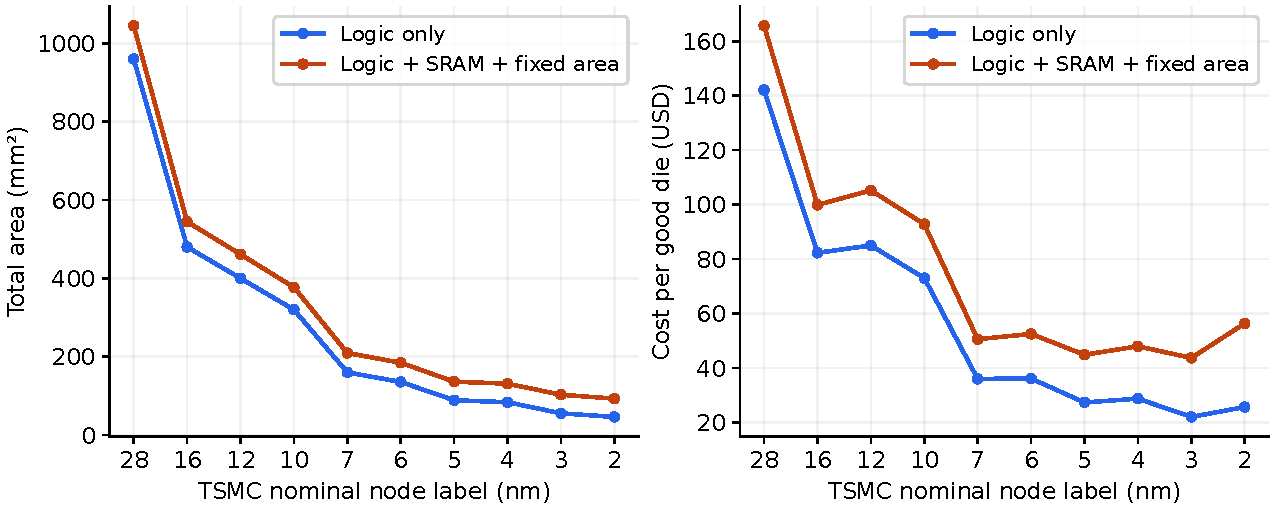
\includegraphics[width=\linewidth]{figures/node_sweep.pdf}
\caption{Effects of SRAM and fixed area on the TSMC sweep. Labels are
categorical process points. Both curves use the same reference logic
design and introductory-price basis. The second scenario adds
256\,Mbit SRAM, 2\,W source SRAM power, and 40\,mm$^2$ fixed area.}
\label{fig:sweep}
\end{figure}

At N3 this second scenario costs \$43.64, increasing to \$56.32 at N2.
Figure~\ref{fig:sweep} illustrates how area that scales slowly or not at
all reduces the economic value of further logic shrinkage. The specific
magnitudes depend on the assumed SRAM macro densities and the decision to
treat fixed blocks as area-only contributions.

\subsection{Cost basis and one-factor sensitivity}
Changing only N6's cost basis from introductory price (\$12,493.50 per
wafer) to manufacturing cost (\$4,024) changes cost per good die from
\$36.07 to \$12.97. Area, power, frequency, and yield remain identical.
This difference measures a modeling convention, not an observed discount.

\begin{table}[htbp]
\centering\small
\caption{One-factor changes around the default N6 case. Baseline values are
135.59\,mm$^2$, 1.20\,GHz, 6.178\,W, 79.03\%, and \$36.07.}
\label{tab:sensitivity}
% Generated by scripts/render_figures.py
\begin{tabular}{lrrrrrr}
\toprule
Parameter & Value & Area & GHz & W & Yield (\%) & Cost (\$)\\
\midrule
Defect multiplier $m_D$ & 0.5 & 135.59 & 1.20 & 6.178 & 86.52 & 33.11 \\
Defect multiplier $m_D$ & 2.0 & 135.59 & 1.20 & 6.178 & 66.45 & 42.52 \\
Wafer multiplier $m_C$ & 0.5 & 135.59 & 1.20 & 6.178 & 79.03 & 19.03 \\
Wafer multiplier $m_C$ & 2.0 & 135.59 & 1.20 & 6.178 & 79.03 & 70.13 \\
Area overhead $h_A$ & 0.8 & 108.47 & 1.20 & 6.129 & 81.92 & 27.95 \\
Area overhead $h_A$ & 1.2 & 162.71 & 1.20 & 6.225 & 76.27 & 44.86 \\
Frequency realization $h_f$ & 0.8 & 135.59 & 0.96 & 5.009 & 79.03 & 36.07 \\
Frequency realization $h_f$ & 1.2 & 135.59 & 1.44 & 7.347 & 79.03 & 36.07 \\
Power guardband $h_P$ & 0.8 & 135.59 & 1.20 & 5.009 & 79.03 & 36.07 \\
Power guardband $h_P$ & 1.2 & 135.59 & 1.20 & 7.347 & 79.03 & 36.07 \\
\bottomrule
\end{tabular}

\end{table}

Table~\ref{tab:sensitivity} reports changes in one parameter at a time.
Doubling the defect multiplier increases cost to \$42.52. A 20\% logic-area
overhead increases cost to \$44.86 through both fewer gross dies and lower
yield. Frequency realization and the logic power guardband affect power
without changing modeled yield or cost. Their equal power effects in this
logic-only case follow from their product in the dynamic term; they need
not be equivalent when SRAM power is present.

The structure of the equations makes local sensitivity explicit. At fixed
geometry, $\alpha$, line yield, wafer cost, and layer count,
\begin{equation}
\frac{\partial\ln C_{\mathrm{Si}}}{\partial D_0}
=\frac{L A_c}{1+D_0 A_c/\alpha},\qquad
\frac{\partial\ln C_{\mathrm{Si}}}{\partial\ln b}=-(L-1).
\end{equation}
The additive package/test and NRE terms reduce the corresponding relative
sensitivity of total delivered-die cost. These derivatives are properties
of the implemented model, not empirically fitted elasticities.

\subsection{Stacking as an assumption study}
To exercise the existing W2W path, we select the repository's Huawei
LogicFold 2026 record under the same N12 reference design. This is a roadmap
scenario with missing primary-source slides, not a claim about a fabricated
Huawei device. The record gives 88.84\,mm$^2$ footprint, 1.879\,GHz, and
16.748\,W, with single-layer post-line yield $q=0.60413$ and
$b=0.995$.

At two layers, modeled stack yield is 36.31\% and cost is \$96.91;
at three layers they become 21.83\% and \$238.84. The selected footprint,
power, and frequency do not change with layer count. Removing the common
\$2 package/test term gives the exact relationship
\begin{equation}
\frac{C_{\mathrm{Si},3}}{C_{\mathrm{Si},2}}=
\frac{3}{2qb}\approx2.495.
\end{equation}
The additional wafer and compounded yield loss explain the increase.
The experiment does not optimize layer partitioning, bonding technology,
interconnect overhead, or thermal behavior.

\subsection{Analytical versus spatial yield}
On first load, the map has independent defaults: 20\,mm square dies,
$D_0=0.28$\,cm$^{-2}$, a \$4,024 wafer, 3\,mm edge exclusion,
PPM=1,000, radial boost $\beta=0.6$, and seed 2026. It reports 148 full
dies, 52 passing dies, and expected yield 32.70\%. This initial map is
not the default N6 analytical scenario.

After target synchronization the dimensions become 11.64\,mm by
11.64\,mm, with $D_0=0.14$ and wafer cost rounded to \$12,494. Retaining
the map's edge and PPM defaults gives 448 full dies, expected yield
76.7839\%, and expected cost \$38.32. Seed 2026 yields 352 passing
dies (78.5714\%) and sampled cost \$37.49. The analytical card gives
79.0286\% and \$36.07, owing to its different geometry, lack of explicit
PPM/radial losses, and unrounded inputs.

Setting only map radial boost and PPM to zero raises expected yield to
79.0394\%, close to the analytical 79.0286\%; the remaining difference is
consistent with rounded die dimensions. Expected map cost remains \$37.28
because its integer placement and explicit edge exclusion still differ
from Eq.~\ref{eq:gross}. Across seeds 1--100 with the synchronized default
map, mean sampled yield is 76.6496\%, with sample standard deviation
1.9500 percentage points and range 70.5357--81.2500\%. The closeness of
the sample mean to 76.7839\% is a sampling sanity check, not a validation
against fab data or a proof of hash independence.

\section{Limitations and validation needs}
The dominant limitation is parameter provenance. Several process factors
are interpolated, costs and defect densities are assumed, and the uploaded
materials referenced by the original interface are absent. The qualitative
confidence labels cannot support a quantitative uncertainty interval.
Published PPA percentages can also describe different voltage, library,
utilization, or iso-power/iso-frequency conditions. Treating them as
independent scalar factors can combine operating points that are not jointly
achievable.

Physical-design effects are represented only by user multipliers. There is
no RTL synthesis, floorplanning, placement, routing, parasitic extraction,
static timing analysis, IR-drop calculation, or thermal simulation.
The model omits IO/analog power, explicit interconnect power, workload
activity traces, SRAM leakage, and memory redundancy. It imposes no reticle
limit and does not optimize die placement. Its negative-binomial law uses
total die area as effective defect-sensitive area.

W2W estimates assume equal layers and independent pass events. The model
does not allocate different circuits to layers, model bonding overhead
cost separately, account for die-to-wafer selection, or characterize
inter-layer correlation. A layer-count increase changes cost and yield
without generating a new physical design. The radial yield map likewise
does not model observed spatial defect clusters.

Arithmetic checks cannot resolve these limitations. A predictive evaluation
would require designs with matched source and target cell libraries,
comparable physical-design constraints, characterized SRAM macros,
measured or signoff-quality power and timing, and sourced yield/cost
assumptions. Calibration designs should be separated from held-out designs.
Such a study could report area, frequency, and power errors individually,
and propagate yield/cost parameter uncertainty. This paper contains no such
dataset, and leaves that evaluation to future work.

\section{Conclusion}
\tool{} provides a compact, inspectable environment for exploring
the relationships between process factors, design composition, yield, and
cost. Its useful distinction is the separation of logic, SRAM, and fixed
area, together with analytical and spatial views of manufacturing
assumptions. The reproduced experiments show how cost-basis selection,
unscaled area, and stacked yield can dominate conclusions drawn from logic
density alone. The artifact supports transparent scenario analysis; its
predictive use requires calibration and independent validation beyond the
repository's default library.

\section*{Artifact availability and acknowledgments}
The repository is distributed under Apache-2.0. This manuscript is accompanied
by its LaTeX source, vector figures, editable draw.io architecture, numerical
results, and reproduction instructions. This documentation and manuscript
draft were prepared with AI assistance. Manuscript content requires author
review before submission.

\begin{thebibliography}{9}
\raggedright
\bibitem{stillmaker2017}
A. Stillmaker and B. M. Baas.
Scaling equations for the accurate prediction of CMOS device performance
from 180 nm to 7 nm.
\emph{Integration, the VLSI Journal}, 58:74--81, 2017.
\href{https://doi.org/10.1016/j.vlsi.2017.02.002}{doi:10.1016/j.vlsi.2017.02.002}.
Author-hosted version and corrigendum:
\url{https://vcl.ece.ucdavis.edu/pubs/2017.02.VLSIintegration.TechScale/}.

\bibitem{deepscale2021}
S. Sarangi and B. Baas.
DeepScaleTool: A tool for the accurate estimation of technology scaling
in the deep-submicron era. 2021.
\url{https://arxiv.org/abs/2102.10195}.

\bibitem{yield2003}
Yu. I. Bogdanov, N. A. Bogdanova, and V. L. Dshkhunyan.
Statistical yield modeling for IC manufacture: Hierarchical fault
distributions. 2003.
\url{https://arxiv.org/abs/physics/0303039}.

\bibitem{tsmc2019}
TSMC. TSMC unveils 6-nanometer process. April 16, 2019.
\url{https://pr.tsmc.com/english/news/1989}.

\bibitem{gf2015}
GlobalFoundries.
GLOBALFOUNDRIES launches industry's first 22nm FD-SOI technology platform.
July 13, 2015.
\url{https://investors.gf.com/news-releases/news-release-details/globalfoundries-launches-industrys-first-22nm-fd-soi-technology}.

\bibitem{gf2018}
GlobalFoundries.
GLOBALFOUNDRIES reshapes technology portfolio to intensify focus on growing
demand for differentiated offerings. August 27, 2018.
\url{https://investors.gf.com/news-releases/news-release-details/globalfoundries-reshapes-technology-portfolio-intensify-focus}.
\end{thebibliography}
\end{document}
